\documentclass[tikz,border=0pt]{standalone}
\usepackage{fontspec}
\IfFontExistsTF{TeX Gyre Heros}{\setmainfont{TeX Gyre Heros}}{\setmainfont{Latin Modern Sans}}
\usepackage{amsmath,amssymb,booktabs,array}
\DeclareMathSizes{9}{9}{8.6}{8.6}
\usepackage{pgfplots}
\pgfplotsset{compat=1.17}
\usetikzlibrary{arrows.meta,positioning,calc,fit,shapes.geometric,backgrounds}
\definecolor{ink}{HTML}{183247}
\definecolor{blue}{HTML}{286B91}
\definecolor{teal}{HTML}{19796F}
\definecolor{orange}{HTML}{AC671F}
\definecolor{muted}{HTML}{596C78}
\tikzset{
  every node/.style={font=\fontsize{9}{11}\selectfont,text=ink},
  arr/.style={-{Stealth[length=1.7mm]},line width=.55pt,draw=muted},
  panel/.style={draw=muted!35,line width=.5pt,rounded corners=1mm,fill=white},
  box/.style={draw=blue!70,line width=.55pt,rounded corners=.8mm,fill=blue!5,align=center,inner sep=2mm},
  label/.style={font=\fontsize{9}{11}\selectfont,align=left,inner sep=0},
  paneltitle/.style={font=\bfseries\fontsize{9.5}{12}\selectfont,anchor=west,inner sep=0}
}

\begin{document}
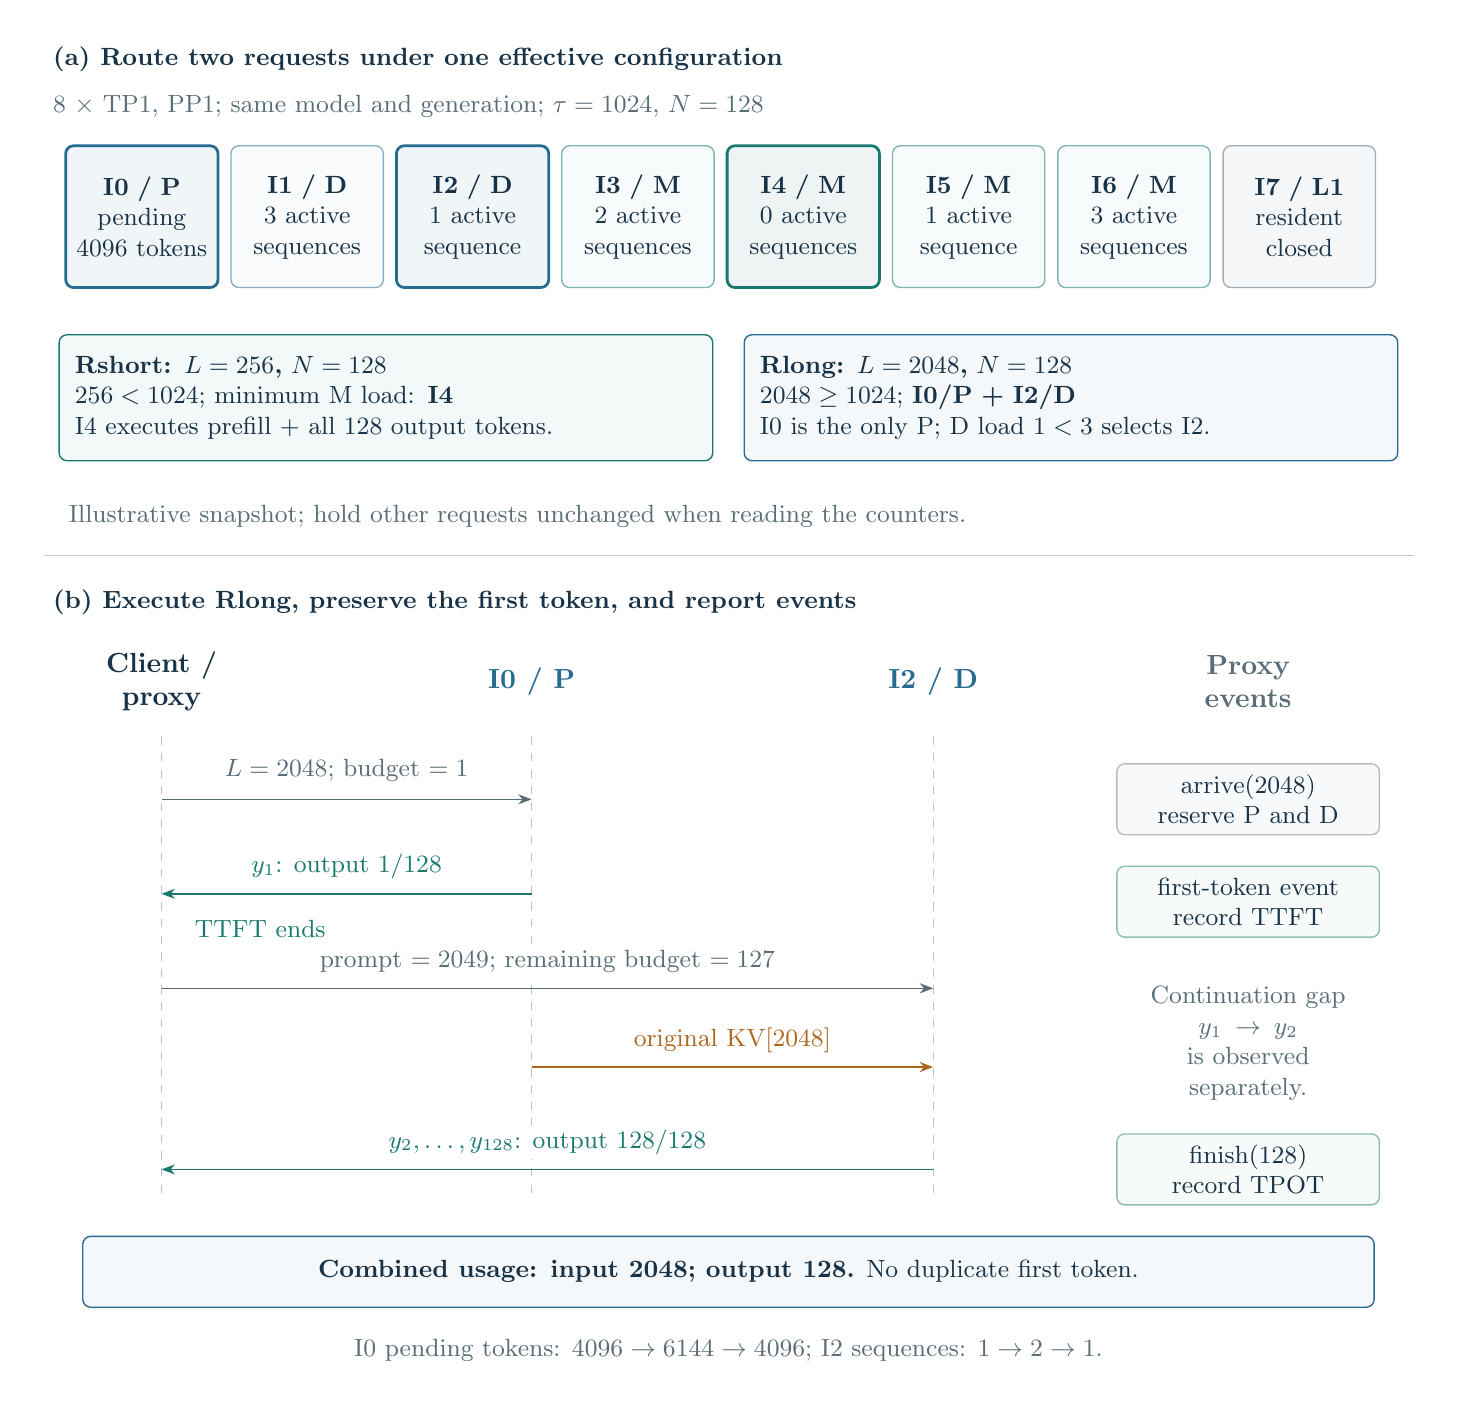
\begin{tikzpicture}[x=1mm,y=-1mm,font=\fontsize{9}{11}\selectfont]
  \path[use as bounding box] (0,0) rectangle (178,172);
  \node[anchor=west,font=\bfseries\fontsize{9}{11}\selectfont,text=ink] at (2,4) {(a) Route two requests under one effective configuration};
  \node[anchor=west,text=muted] at (2,10) {8 $\times$ TP1, PP1; same model and generation; $\tau=1024$, $N=128$};

  \node[panel,draw=blue,line width=1pt,fill=blue!7,minimum width=19mm,minimum height=18mm,align=center,text width=17mm] at (14.5,24) {\textbf{I0 / P}\\pending\\4096 tokens};
  \node[panel,draw=blue!55,fill=blue!3,minimum width=19mm,minimum height=18mm,align=center,text width=17mm] at (35.5,24) {\textbf{I1 / D}\\3 active\\sequences};
  \node[panel,draw=blue,line width=1pt,fill=blue!7,minimum width=19mm,minimum height=18mm,align=center,text width=17mm] at (56.5,24) {\textbf{I2 / D}\\1 active\\sequence};
  \node[panel,draw=teal!55,fill=teal!3,minimum width=19mm,minimum height=18mm,align=center,text width=17mm] at (77.5,24) {\textbf{I3 / M}\\2 active\\sequences};
  \node[panel,draw=teal,line width=1pt,fill=teal!8,minimum width=19mm,minimum height=18mm,align=center,text width=17mm] at (98.5,24) {\textbf{I4 / M}\\0 active\\sequences};
  \node[panel,draw=teal!55,fill=teal!3,minimum width=19mm,minimum height=18mm,align=center,text width=17mm] at (119.5,24) {\textbf{I5 / M}\\1 active\\sequence};
  \node[panel,draw=teal!55,fill=teal!3,minimum width=19mm,minimum height=18mm,align=center,text width=17mm] at (140.5,24) {\textbf{I6 / M}\\3 active\\sequences};
  \node[panel,draw=muted!55,fill=muted!6,minimum width=19mm,minimum height=18mm,align=center,text width=17mm] at (161.5,24) {\textbf{I7 / L1}\\resident\\closed};

  \node[panel,draw=teal,fill=teal!5,minimum width=83mm,minimum height=16mm,align=left,text width=79mm] at (45.5,47) {\textbf{Rshort: $L=256$, $N=128$}\\$256<1024$; minimum M load: \textbf{I4}\\I4 executes prefill + all 128 output tokens.};
  \node[panel,draw=blue,fill=blue!5,minimum width=83mm,minimum height=16mm,align=left,text width=79mm] at (132.5,47) {\textbf{Rlong: $L=2048$, $N=128$}\\$2048\geq1024$; \textbf{I0/P + I2/D}\\I0 is the only P; D load $1<3$ selects I2.};
  \node[anchor=west,text=muted] at (4,62) {Illustrative snapshot; hold other requests unchanged when reading the counters.};

  \draw[muted!35] (2,67) -- (176,67);
  \node[anchor=west,font=\bfseries\fontsize{9}{11}\selectfont,text=ink] at (2,73) {(b) Execute Rlong, preserve the first token, and report events};
  \node[font=\bfseries,text=ink,align=center] at (17,83) {Client /\\proxy};
  \node[font=\bfseries,text=blue] at (64,83) {I0 / P};
  \node[font=\bfseries,text=blue] at (115,83) {I2 / D};
  \node[font=\bfseries,text=muted,align=center] at (155,83) {Proxy\\events};
  \foreach \x in {17,64,115} {\draw[muted!40,dashed] (\x,90) -- (\x,149);}

  \draw[arr] (17,98) -- (64,98);
  \node[fill=white,inner sep=0.6mm,text=muted] at (40.5,94.3) {$L=2048$; budget $=1$};
  \node[panel,draw=muted!45,fill=muted!4,align=center,text width=31mm,minimum height=9mm] at (155,98) {arrive(2048)\\reserve P and D};

  \draw[arr,draw=teal] (64,110) -- (17,110);
  \node[fill=white,inner sep=0.6mm,text=teal] at (40.5,106.5) {$y_1$: output $1/128$};
  \node[anchor=west,text=teal] at (20,114.5) {TTFT ends};
  \node[panel,draw=teal!50,fill=teal!4,align=center,text width=31mm,minimum height=9mm] at (155,111) {first-token event\\record TTFT};

  \draw[arr] (17,122) -- (115,122);
  \node[fill=white,inner sep=0.6mm,text=muted] at (66,118.6) {prompt $=2049$; remaining budget $=127$};

  \draw[arr,draw=orange,line width=1pt] (64,132) -- (115,132);
  \node[fill=white,inner sep=0.6mm,text=orange] at (89.5,128.6) {original KV[2048]};
  \node[align=center,text=muted,text width=31mm] at (155,129) {Continuation gap\\$y_1\!\rightarrow\!y_2$\\is observed separately.};

  \draw[arr,draw=teal] (115,145) -- (17,145);
  \node[fill=white,inner sep=0.6mm,text=teal] at (66,141.5) {$y_2,\ldots,y_{128}$: output $128/128$};
  \node[panel,draw=teal!50,fill=teal!4,align=center,text width=31mm,minimum height=9mm] at (155,145) {finish(128)\\record TPOT};

  \node[panel,draw=blue,fill=blue!5,minimum width=164mm,minimum height=9mm,align=center] at (89,158) {\textbf{Combined usage: input 2048; output 128.} No duplicate first token.};
  \node[align=center,text=muted] at (89,168) {I0 pending tokens: $4096\to6144\to4096$; I2 sequences: $1\to2\to1$.};
\end{tikzpicture}
\end{document}
